\documentclass{report}
\usepackage{amsmath}
\usepackage{bm}
\usepackage{colortbl}
\usepackage{graphicx}
\usepackage{fullpage}
\usepackage{multirow}
\usepackage{setspace}
\usepackage{booktabs}
\usepackage{gensymb}
\usepackage{xr}
\usepackage[inline]{enumitem}
\usepackage[natbib=true, style=numeric-comp,subentry,backend=biber,sorting=none]{biblatex}
\addbibresource{citation/Thesis.bib}
\usepackage[hidelinks]{hyperref}
\usepackage{fancyhdr}
\pagestyle{fancy}
\fancyhead[LE,RO]{\itshape \nouppercase \rightmark}
\fancyhead[LO,RE]{\itshape \nouppercase Chapter \arabic{chapter}}
\setlength{\headheight}{40.0pt}
\setlength{\headsep}{0.2in}
\addtolength{\topmargin}{-4\baselineskip}


\title{Thesis outline \\
\large Genetic and Environmental risk factors of Neurodevelopmental disorders}
\date{\today}
\author{Choi Shing Wan}
\renewcommand*\contentsname{Table of Content}

\newcommand{\gene}[1]{\textit{#1}}
\newcommand{\organism}[1]{\textit{#1}}
\newcommand{\function}[1]{\textit{#1}}
\begin{document}
\maketitle
\chapter*{Declaration}
\chapter*{Acknowledgements}
\tableofcontents

 \onehalfspacing
\chapter{General Introduction and literature review (What has been done)}
\section{Neurodevelopmental disorders}
\subsection{Schizophrenia}
\subsection{Autism}

To understand these disorders, researchers conduct different studies
\section{Contribution of Genetic and Environmental risk factors}
\subsection{Epidemiological studies}
Looking into records
Find out what is common between the people
e.g. alcohol use, prenatal infection

Here we will discuss how different environmental risk factors were considered as risk factors for neurodevelopmental disorders (e.g. Etiological studies)
\subsection{Postnatal stress}
\subsection{Maternal use of alcohol}
\subsection{Socio-economical status}
\subsection{Maternal immune activation}
At the end, we would like to comparing different environmental risk factors and then say that maternal immune activation were the most interested as this is the single biggest risk factor

\subsection{Twin Studies}
Only small amount of similarity between the environmental factors
Will there be anything other than environment?
Use twins studies to find out.

\section{Genetic Risk Factors}
Now we know genetic is the main factor, how to study it?
And also how people study the role of genetics in a disease.
So basically, will have brief discussion on gwas, exome sequencing and whole genome sequencing
\subsection{Common Single Nucleotide Polymorphism}
\subsubsection{Genome-wide association studies}
\subsection{Rare Single Nucleotide Mutation}
\subsection{Copy Number Variation (CNV)}

\section{Aim of the study}
\paragraph{} In this thesis



\chapter{Environmental risk factors of Neurodevelopmental disorders}
\section{Introduction}
Briefly say that environmental risk are interesting to study because one might prevent said environment to prevent the disorder. 
\subsection{Maternal Immune activation}
Environmental insults, such as infections during the prenatal period, have a negative impact on the normal course of fetal brain development.
The consequences of postnatal brain dysmaturation\cite{Meyer2007a} include an increased risk of neurodevelopmental conditions such as  schizophrenia and autism \cite{Fatemi2009a,Bale2010}. 
Prenatal infection and Maternal immune activation (MIA) can be modeled in the rodent; specifically the viral analogue polyriboinosinic-polyribocytidilic acid (PolyI:C) precipitates a brain and behavioral phenotype in rodent offspring which mirrors that observed in schizophrenia and related neurodevelopmental conditions\cite{Li2009c,Meyer2008b,Li2010a,Ashwood2006}.

Recent studies of global gene expression patterns in MIA-exposed rodent fetal brains\cite{Garbett2012,Oskvig2012} suggest that the post-pubertal onset of schizophrenic and other psychosis-related phenotypes might stem from attempts of the brain to counteract the environmental stress induced by MIA during its early development\cite{Garbett2012}.
To date, all these studies have focused on the changes elicited by a mid-to-late gestation exposure (e.g. Gestation Day (GD) 12.5 for mouse, or GD15 for rat). 
However, although we and others\cite{Meyer2007a,Li2009c,Li2010a} have reported that MIA early in gestation event might exert a more extensive impact on the phenotype of offspring, gene expression changes soon after early MIA have not been examined. 

This early time point was therefore the focus of the present pilot study. 
We exploited recent advances in transcriptome analysis facilitated by RNA Sequencing (RNA-Seq) to obtain a profile of all expressed transcripts in embryonic brains of mice exposed to early MIA - an approach considered to be more accurate and reliable compared to conventional microarrays\cite{Wang2009b}.
Also, as Proof of Concept, we examined whether the gene expression changes in the MIA model mapped to gene implicated in schizophrenia and autism in humans.

\subsubsection{Immediate effect of maternal immune activation to gene expression pattern in foetal brain}
Here we further discuss how we focus on the current study: The immediate effect of MIA and also the effect of MIA during early gestation. 
Can follow some of the logic from the paper

\subsection{RNA Sequencing}
Discuss the use of RNA Sequencing, comparing with micro-array. 
\subsubsection{Different dimension of the transcriptom}
Should discuss all possible dimention of the RNA Seq data. 
Didn't include miRNA as they are not captured.
Should also mention Alternative splicing, fusion genes and denovo assembly.
\paragraph{Differential Gene Expression}
\paragraph{Alternative Splicing}
\paragraph{Fusion Genes}
\paragraph{Denovo transcripts}
Then should mention the problem of the analysis of Alternative splicing, fusion genes and denovo assembly:
Require large amount of wet lab validation in order to make sense of the data.
Our study is only a pilot study, therefore focus only on the differential expression analysis. 
\subsection{Aim}


\section{Material and Methods}
%\externaldocument{environmental_risk/er_rtPCR_primer.tex}

\subsection{Mouse model}
\subsubsection{Sample Collection}
Two pregnant female C57BL/6N mice were obtained from the University of Hong Kong Laboratory Animal Unit (HKU-LAU).
Both animals were housed at standard temperature (21$\pm$1\degree C ) and humidity (55$\pm$5$\%$ ) under normal light-dark conditions (12 hours light/12 hours dark with lights on between 7:00 and 19:00).
Food and water were available \textit{ad lib}.
All experimental protocols were approved by the Committee on the Use of Live Animals in Teaching and Research at \gls{hku} (CULATAR 3070-13) and also from the Department of Health, Hong Kong Special Administrative Region (12-731) and were carried out in accordance with the approved guidelines. 

The day on which the vaginal plug was found was designated as \gls{gd} 0.
On \gls{gd} 9, one pregnant mouse was randomly assigned as case and received a single dose of \gls{polyic} (5mg/kg) via the tail vein under mild physical restraint, whereas the control mouse received a single dose of 0.9$\%$ saline (5ml/kg) \citep{Li2009c}.
The pregnant dams were sacrificed by cervical dislocation, 6 hours after the injection and fetuses were extracted individually.
A cut was made posterior to the fourth ventricles under the dissecting microscope to separate the head of each fetus \citep{Kaufman1992}, which was then frozen immediately in liquid nitrogen until RNA extraction. 


\citet{Meyer2006b} demonstrated that \gls{polyic} administration will leads to a marked increase in maternal serum cytokine levels of IL-1$\beta$, IL-6, IL-10 and TNF-$\alpha$.
Starting from 3 hours after the injection, it was observed that the fetal brain IL-6 level significantly increases and a marked decrease of fetal IL-1$\beta$ level was also observed. 
6 hours after the injection, the level of IL-6 remains elevated with the IL-1$\beta$ become significantly elevated when compare to that of the control samples.
Interestingly, this change is only observed in the \gls{gd}9 samples but not the \gls{gd}17 samples, suggesting that to be a specific change relevant to \gls{gd}9.
Thus, we selected the 6 hour time point for the fetal brain extraction in the hope to observe the immediate effect of PolyI:C insult to the fetal brain expression pattern.

\subsubsection{DNA Extraction and Foetal Sexing}
As a pilot study, we would like to focus our analysis only on the male fetus.
However, due to the early gestation day, where the genital system of the mouse has yet developed, sexing becomes almost impossible using the genital method.
To identify the sex of the fetus, \gls{pcr} were performed on genes presented on the sex chromosomes (XY) based on the protocol suggested by \citet{Clapcote2005a} to determine the sex of the fetus. 
Genomic DNA was extracted from the bodies of the fetuses, which were kept separately, using the TIANamp Genomic DNA kit (Tiangen, Cat. no. DP304) following the manufacturer's instructions.
The fetuses were then sexed by \gls{pcr} using primers as described in \citet{Clapcote2005a}.
 7 out of 10 fetuses from the \gls{polyic} dam and 5 out of 8 fetuses from the Saline dam were male.


\subsection{RNA Sequencing}
\subsubsection{RNA Extraction, Library Construction and Sequencing}
Total RNA was extracted from each fetal brain using RNeasx10-Micro-Kit (Qiagen, Cat. No. 74004) following the manufacturer’s instructions. 
RNA quality was assayed using the Agilent 2100 Bioanalyzer and RNA was quantified using the Qubit 1.0 Fluorometer. 
Samples with an \gls{rin} $\ge$ 9.5 were selected for sequencing (5 cases, 5 controls). 
The RNA-Seq library was performed at the Centre for Genomic Sciences, HKU, using the TruSeq Stranded mRNA Sample Prep Kit. 
The \gls{ercc} spike-in control \citep{Jiang2011a} was included as an internal control. 
All samples were sequenced using Illumina Hiseq at two lanes (2 $\times$ 101 bp paired-end reads) at Macrogen.

\subsubsection{Differential Gene Expression Analysis and Functional Enrichment}
%Should I also compare the performance of different alignment tools and DE analysis tools?

The sequence reads were subject to \gls{qc} using FastQC \citep{Andrews} and mapped to the \textit{Mus musculus} reference genome (mm10, Ensembl GRCm38.74) and ERCC reference using the STAR aligner (version 2.3.1v) \citep{Dobin2013}.
The read count per gene for each sample was calculated with HTseq (version 0.5.4p5) \citep{Anders2015}.
Differential gene expression analysis was performed using the DESeq2 package (version 2.1.4.5) \citep{Anders2010}.
In order to reduce noise associated with low expression, genes with base mean count $<$ 10 were removed from all analyses.
Outliers were replaced using the \textit{replaceOutliersWithTrimmedMean} function in DESeq2 \citep{Anders2010}. 
Genes with p-value passing the Bonferroni corrected p-value $<$ 0.05 were defined as \glspl{deg}. 

\gls{go} based enrichment analysis of \glspl{deg} was performed using GOrilla \citep{Eden2009}, which takes a list of \glspl{deg} as input and tests whether a particular \gls{go} term is overrepresented in the input list when compared to the background gene list.
Up-regulated and down-regulated gene lists were input separately such that we may identify \gls{go} terms corresponding to the up- and down-regulated gene lists.
As GO terms tends to be redundant and overlaps with each other, it will aid the interpretation of GO results based by clustering and reducing the GO terms based on their similarity. 
Thus, \gls{go} enrichment results were summarized by REViGO \citep{Supek2011} and significant representative \gls{go} terms were obtained.
Gene set enrichment analysis was conducted using the \textit{userListEnrichment} \citep{Miller2011} function in R to identify known brain-related gene sets enriched by the DEGs.
A description of these brain-related gene sets can be found in \url{http://www.inside-r.org/packages/cran/WGCNA/docs/userListEnrichment}.
Only gene sets with a Bonferroni corrected p-value $<$ 0.05 were considered as significant. 

\subsection{Combining with External Microarray Controls}
%Need to explain why we perform this analysis
We repeated all analyses mentioned above using control microarrays \gls{gd}9 C57BL/6 mouse fetal brain expression data (N=5) from \gls{geo} (GSE8091 \citep{Hartl2008}) obtained using GEOquery (version 2.30.0) \citep{Davis2007}.
In order to remove effects due to platform differences, our RNA-Seq data was first variance stabilized (\textit{varianceStabilizingTransformation} function in DESeq2\cite{Anders2010}) and then combined with the \textit{rma} normalized microarray data using the Combat algorithm \citep{Johnson2007} under the sva package (version 3.10.0) in R.
Scripts used in all analyses are available online at \url{https://github.com/choishingwan/RNA-Seq-Analysis}. 

\subsection{Burden of Genetic Risk Variants in Brain-Related Gene Sets}
To establish the Proof of Concept that the enriched brain-related gene sets discovered are relevant to schizophrenia and other neuropsychiatric diseases in humans, we tested for 
\begin{enumerate*}[label=\roman*)]
	\item whether there was an excess of reported \textbf{rare} \textit{de novo} genetic mutations in these gene sets in previous studies of autism and schizophrenia patients \citep{Fromer2014,ORoak2012,Sanders2012,Neale2012} using a hyper geometric test; and
	\item whether there was greater evidence of association of \textbf{common} genetic variants with schizophrenia \citep{Ripke2013} and autism \citep{Anney2010a} in these gene sets then in the genome as a whole using a set analysis algorithm \citep{Ideker2002}. 
\end{enumerate*}
Briefly, p-values of genes were first converted into a z-score $z_i$. 
To produce the z-score for each individual gene sets, we sum the z-score within each individual gene sets $z_{gene\ set} = \sum_i^kz_i$ where $k$ is the number of genes within the specific gene set. 
To obtain the background distribution, we construct 10,000 random gene sets of size $k$ using permutation. 
We can then calculate the mean $z_\mu$ and standard deviation $z_\sigma$ of z-score for gene sets of size $k$.
Therefore, we can calculate the significance of enrichment of the gene set as
$$
S_{gene\ set}=\frac{z_{gene\ set}-z_\mu}{z_\sigma}
$$
Which allow us to obtain the p-value using $S_{gene\ set}$. 
The script for this analysis can be also be found at \url{https://github.com/choishingwan/RNA-Seq-Analysis}. 


\subsection{Real time PCR (RT-PCR) validation}
We validated the RNA-Seq results using \gls{rtpcr} on the same samples plus six additional samples from two independent dams (Saline = 8, PolyI:C = 8).
Unfortunately, due to the small tissue size, there were only enough materials for 5 genes for \gls{rtpcr}. 
Therefore, 4 \glspl{deg} (\textit{Akt3}, \textit{Eomes}, \textit{Lama5} and \textit{Robo3}), together with the reference $\beta$-Actin(\textit{Actb}) were selected. 
Primers (designed by Invitrogen) are listed in Table \cref{suppleTab:rtPCR}. 
cDNA was synthesized using SuperScript III reverse transcriptase (Invitrogen). 
RT- PCR was performed by using 2$\mu$l of cDNA product in each reaction on the ABI prism 7900HT Sequence Detection System.
All reactions were run in triplicate and \gls{ct} values for the four genes were normalized with $\beta$-Actin (\textit{Actb}) as the reference. 
A Student’s T-test was performed to compare the normalized \gls{ct} values between the \gls{polyic} fetuses and the saline fetuses for each of the four genes \citep{Yuan2006}.

\section{Result}
\subsection{Quality Control and Alignment}
Figure \ref{fig:schematicMIA} summarizes the overall study design and results obtained.
On average, 39 million reads were generated for each sample. 
Over 90$\%$ of reads were uniquely mapped to the \textit{Mus musculus} reference genome (mm10, Ensembl GRCm38.74) and the ERCC spike-in control reference using STAR\cite{Dobin2013}. 
Read counts of the External RNA Controls Consortium (ERCC) spike-in control were highly correlated with their true concentration (Pearson’s R $\le$ 0.956)(Table \ref{tab:ercc_correlation}), indicating that the RNA Seq read counts were representative of the true mRNA concentration.
\begin{figure}[htbp]
	\centering
	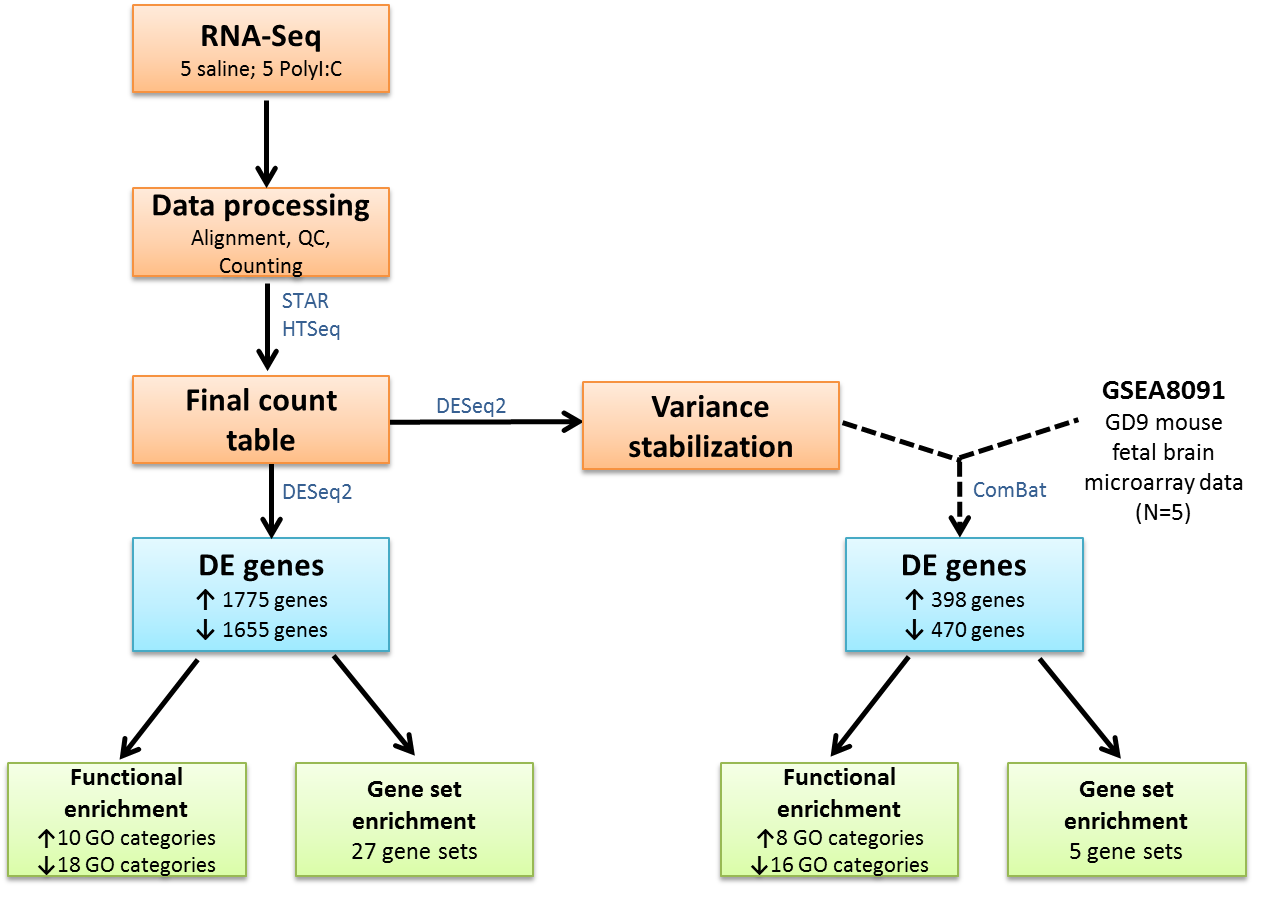
\includegraphics[width=0.9\textwidth]{environmental_risk/image/er_flowchart.png}
	\caption[Schematic of the experimental flow]{Schematic of the experimental flow. 
		Fetal mouse brains were extracted and used for RNA Sequencing. 
		DESeq2 were used to generate the differential expressed gene (DEG) list and also stabilize the variance of the gene expression counts. 
		Functional enrichment analysis were then performed on the DEG list using GOrilla, REViGO and the userListEnrichment function. 
		Stabilzed gene counts were then merged with the external microarray control using ComBat where the differential expression analysis and functional enrichment were again performed}\label{fig:schematicMIA}
\end{figure}
\begin{table}[h]
	\centering
	\caption[Correlation between concentration and counts]{Correlation between the true concentration and the normalized RNA Seq read counts.
		The high correlation indicates that the RNA Seq read counts are representative of the true concentration.}
	\label{tab:ercc_correlation}
	\begin{tabular}{rr}
		\toprule
		& \textbf{True Concentration} \\
		\midrule
		\textbf{Case 1} & 0.964 \\
		\textbf{Case 2} & 0.969 \\
		\textbf{Case 3} & 0.968 \\
		\textbf{Case 4} & 0.960 \\
		\textbf{Case 5} & 0.963 \\
		\textbf{Control 1} & 0.967 \\
		\textbf{Control 2} & 0.964 \\
		\textbf{Control 3} & 0.960 \\
		\textbf{Control 4} & 0.959 \\
		\textbf{Control 5} & 0.966 \\
		\bottomrule
	\end{tabular}%
\end{table}
\\
\\



\subsection{Differential gene expression analysis}
A total of 16,015 genes passed QC, of which 3,430 genes were differentially expressed (1,775 up-regulated and 1,655 down-regulated) with a Bonferroni-corrected p-value $<$ 0.05. 
A volcano plot of PolyI:C versus Saline for all genes is presented in Figure \ref{subfig1:deseqVoc}, with the significantly up- and down-regulated genes colored in red and blue, respectively. 
Many of our differentially expressed genes (DEGs) were within the list of schizophrenia-related candidate genes identified by the Psychiatric Genomics Consortium (PGC)\cite{Greenwood2011} previously (hyper geometric p-value $= 1.12\times 10^{-11}$) (Table \ref{tab:candidateGeneTable}), including \textit{Dlg4}\cite{Balan2013} and \textit{Disc1}\cite{Morris2003}.
Some DEGs were also known to be associated with autism (like \textit{Gabrb3}\cite{Fatemi2009}) or other brain diseases (like \textit{Chrnb2} in epilepsy\cite{Conti2015}).
\begin{figure}[!h]
	\centering     
	\subfloat[Using only RNA Seq data\label{subfig1:deseqVoc}]{%
		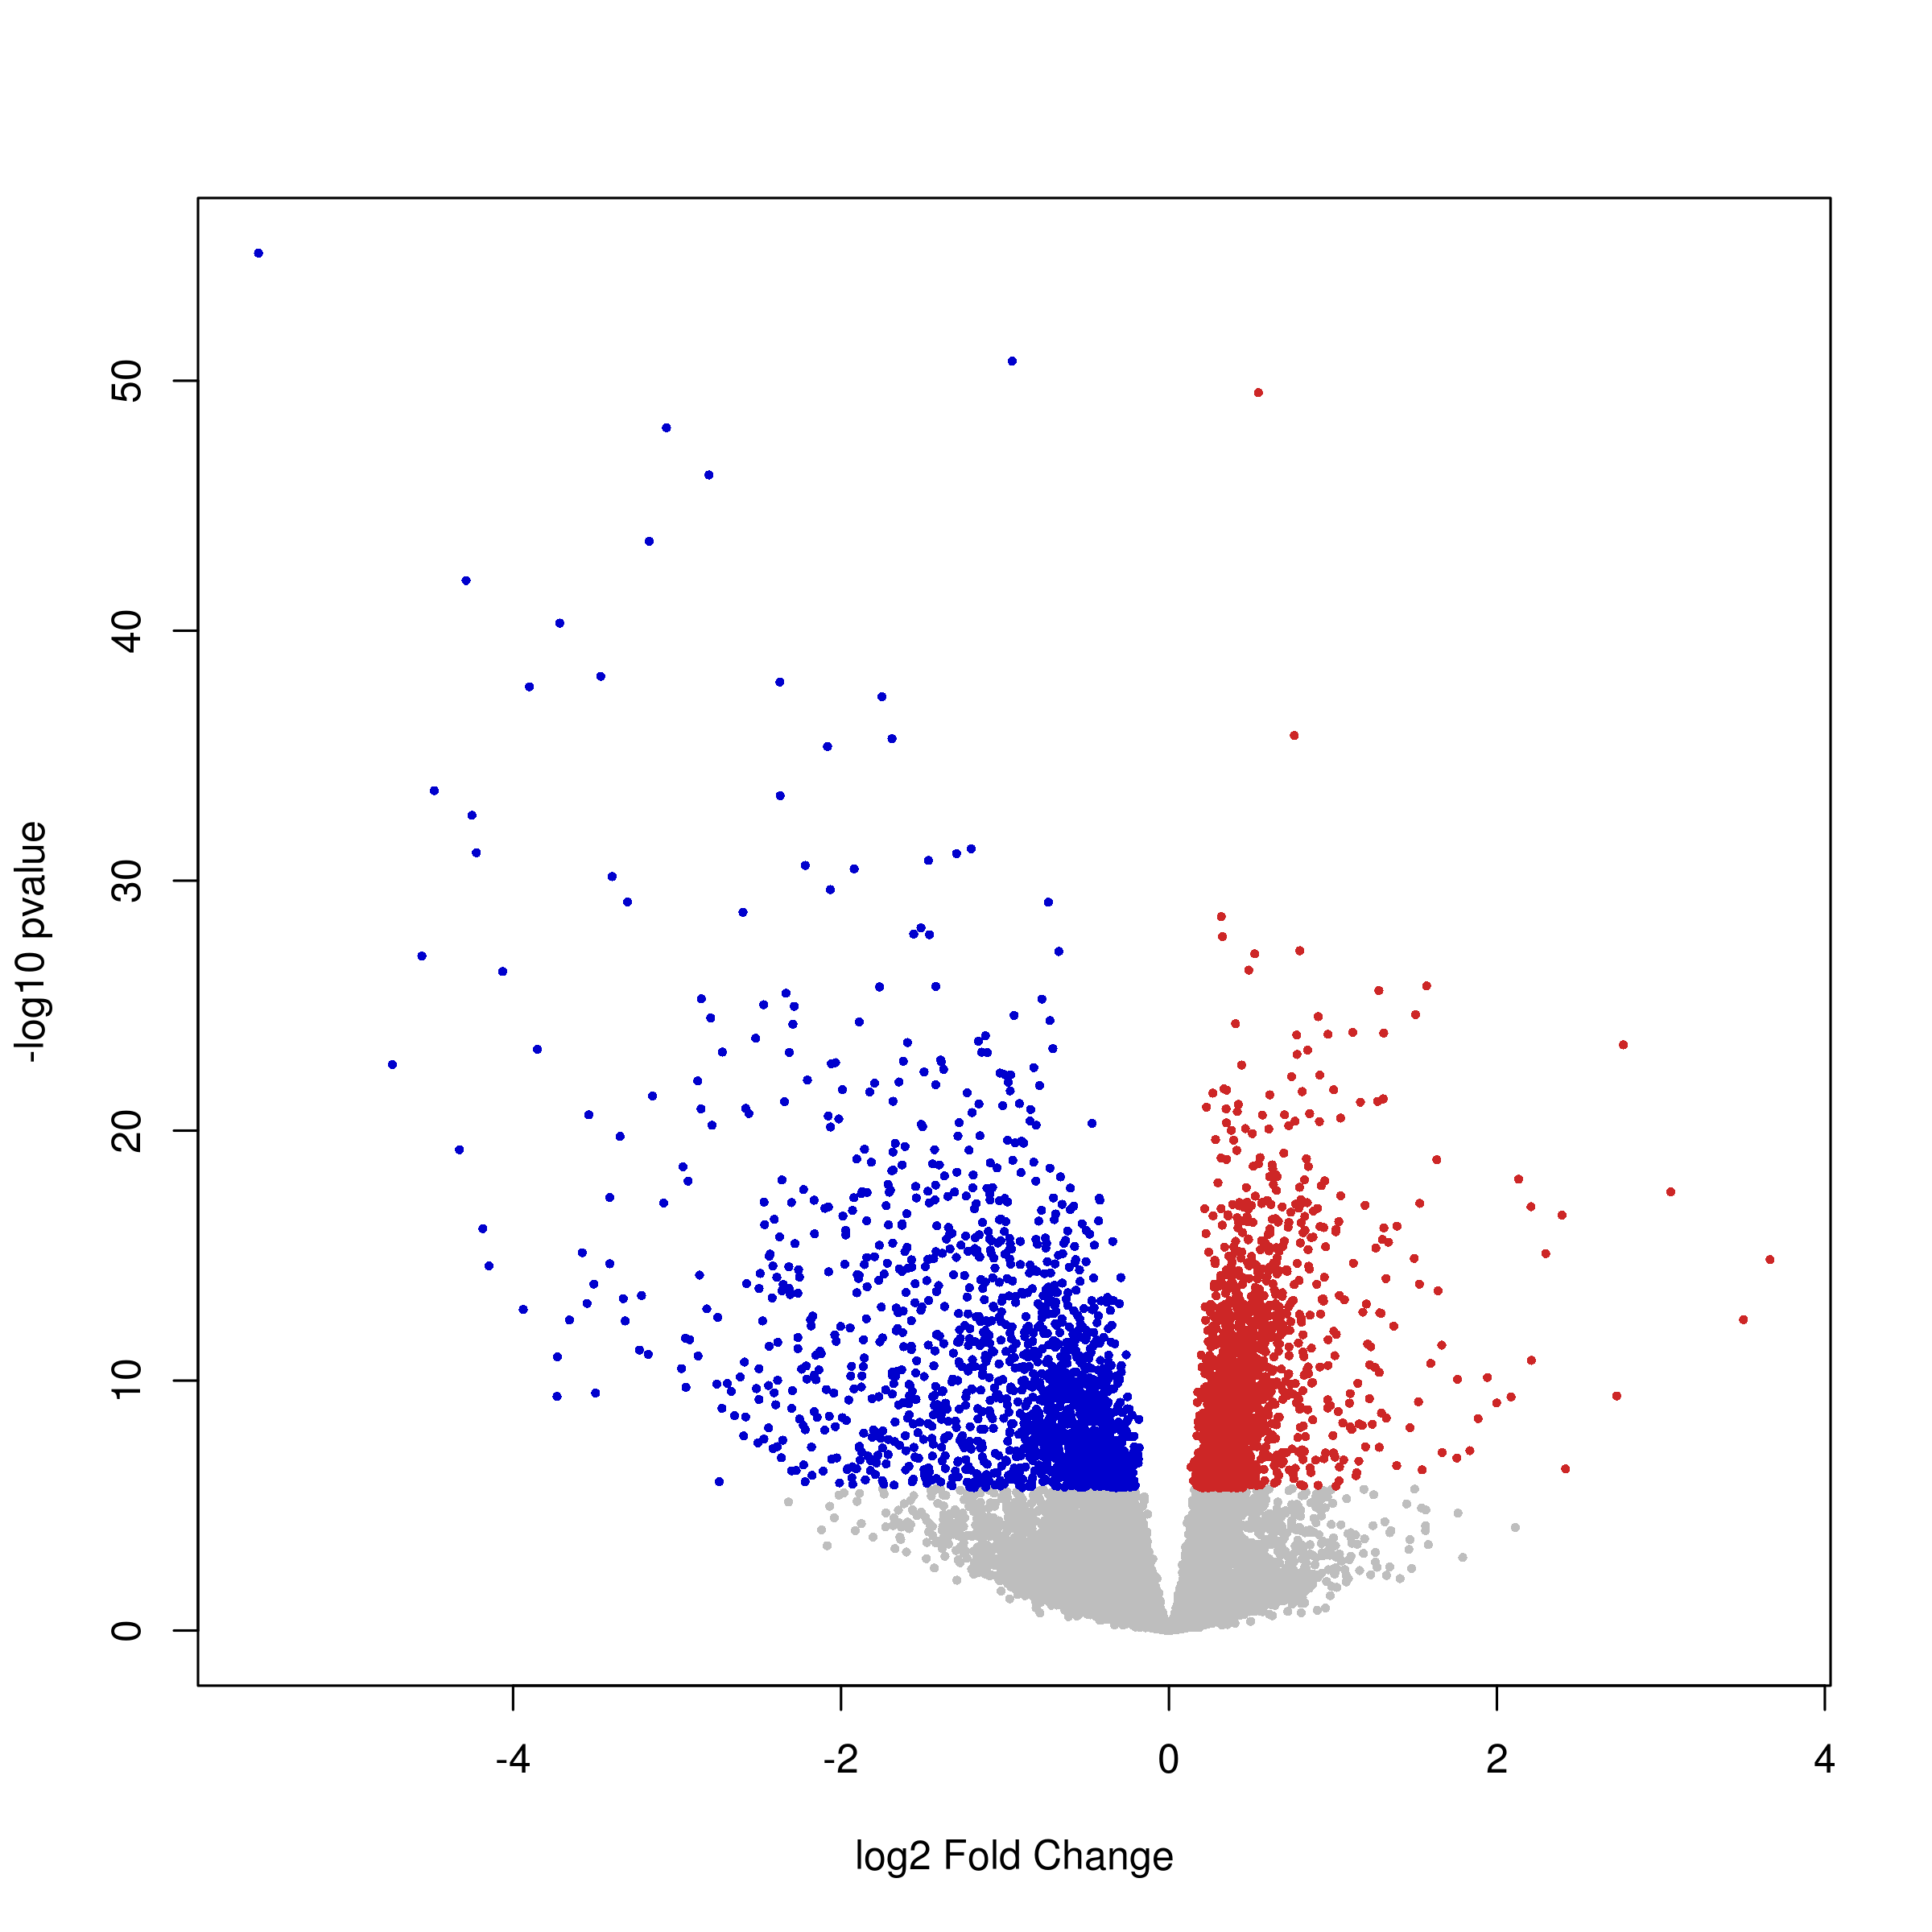
\includegraphics[width=0.45\textwidth]{environmental_risk/image/er_deseq_volcano.png}
	}
	\subfloat[Combining RNA Seq and microarray data\label{subfig2:combatVoc}]{%
		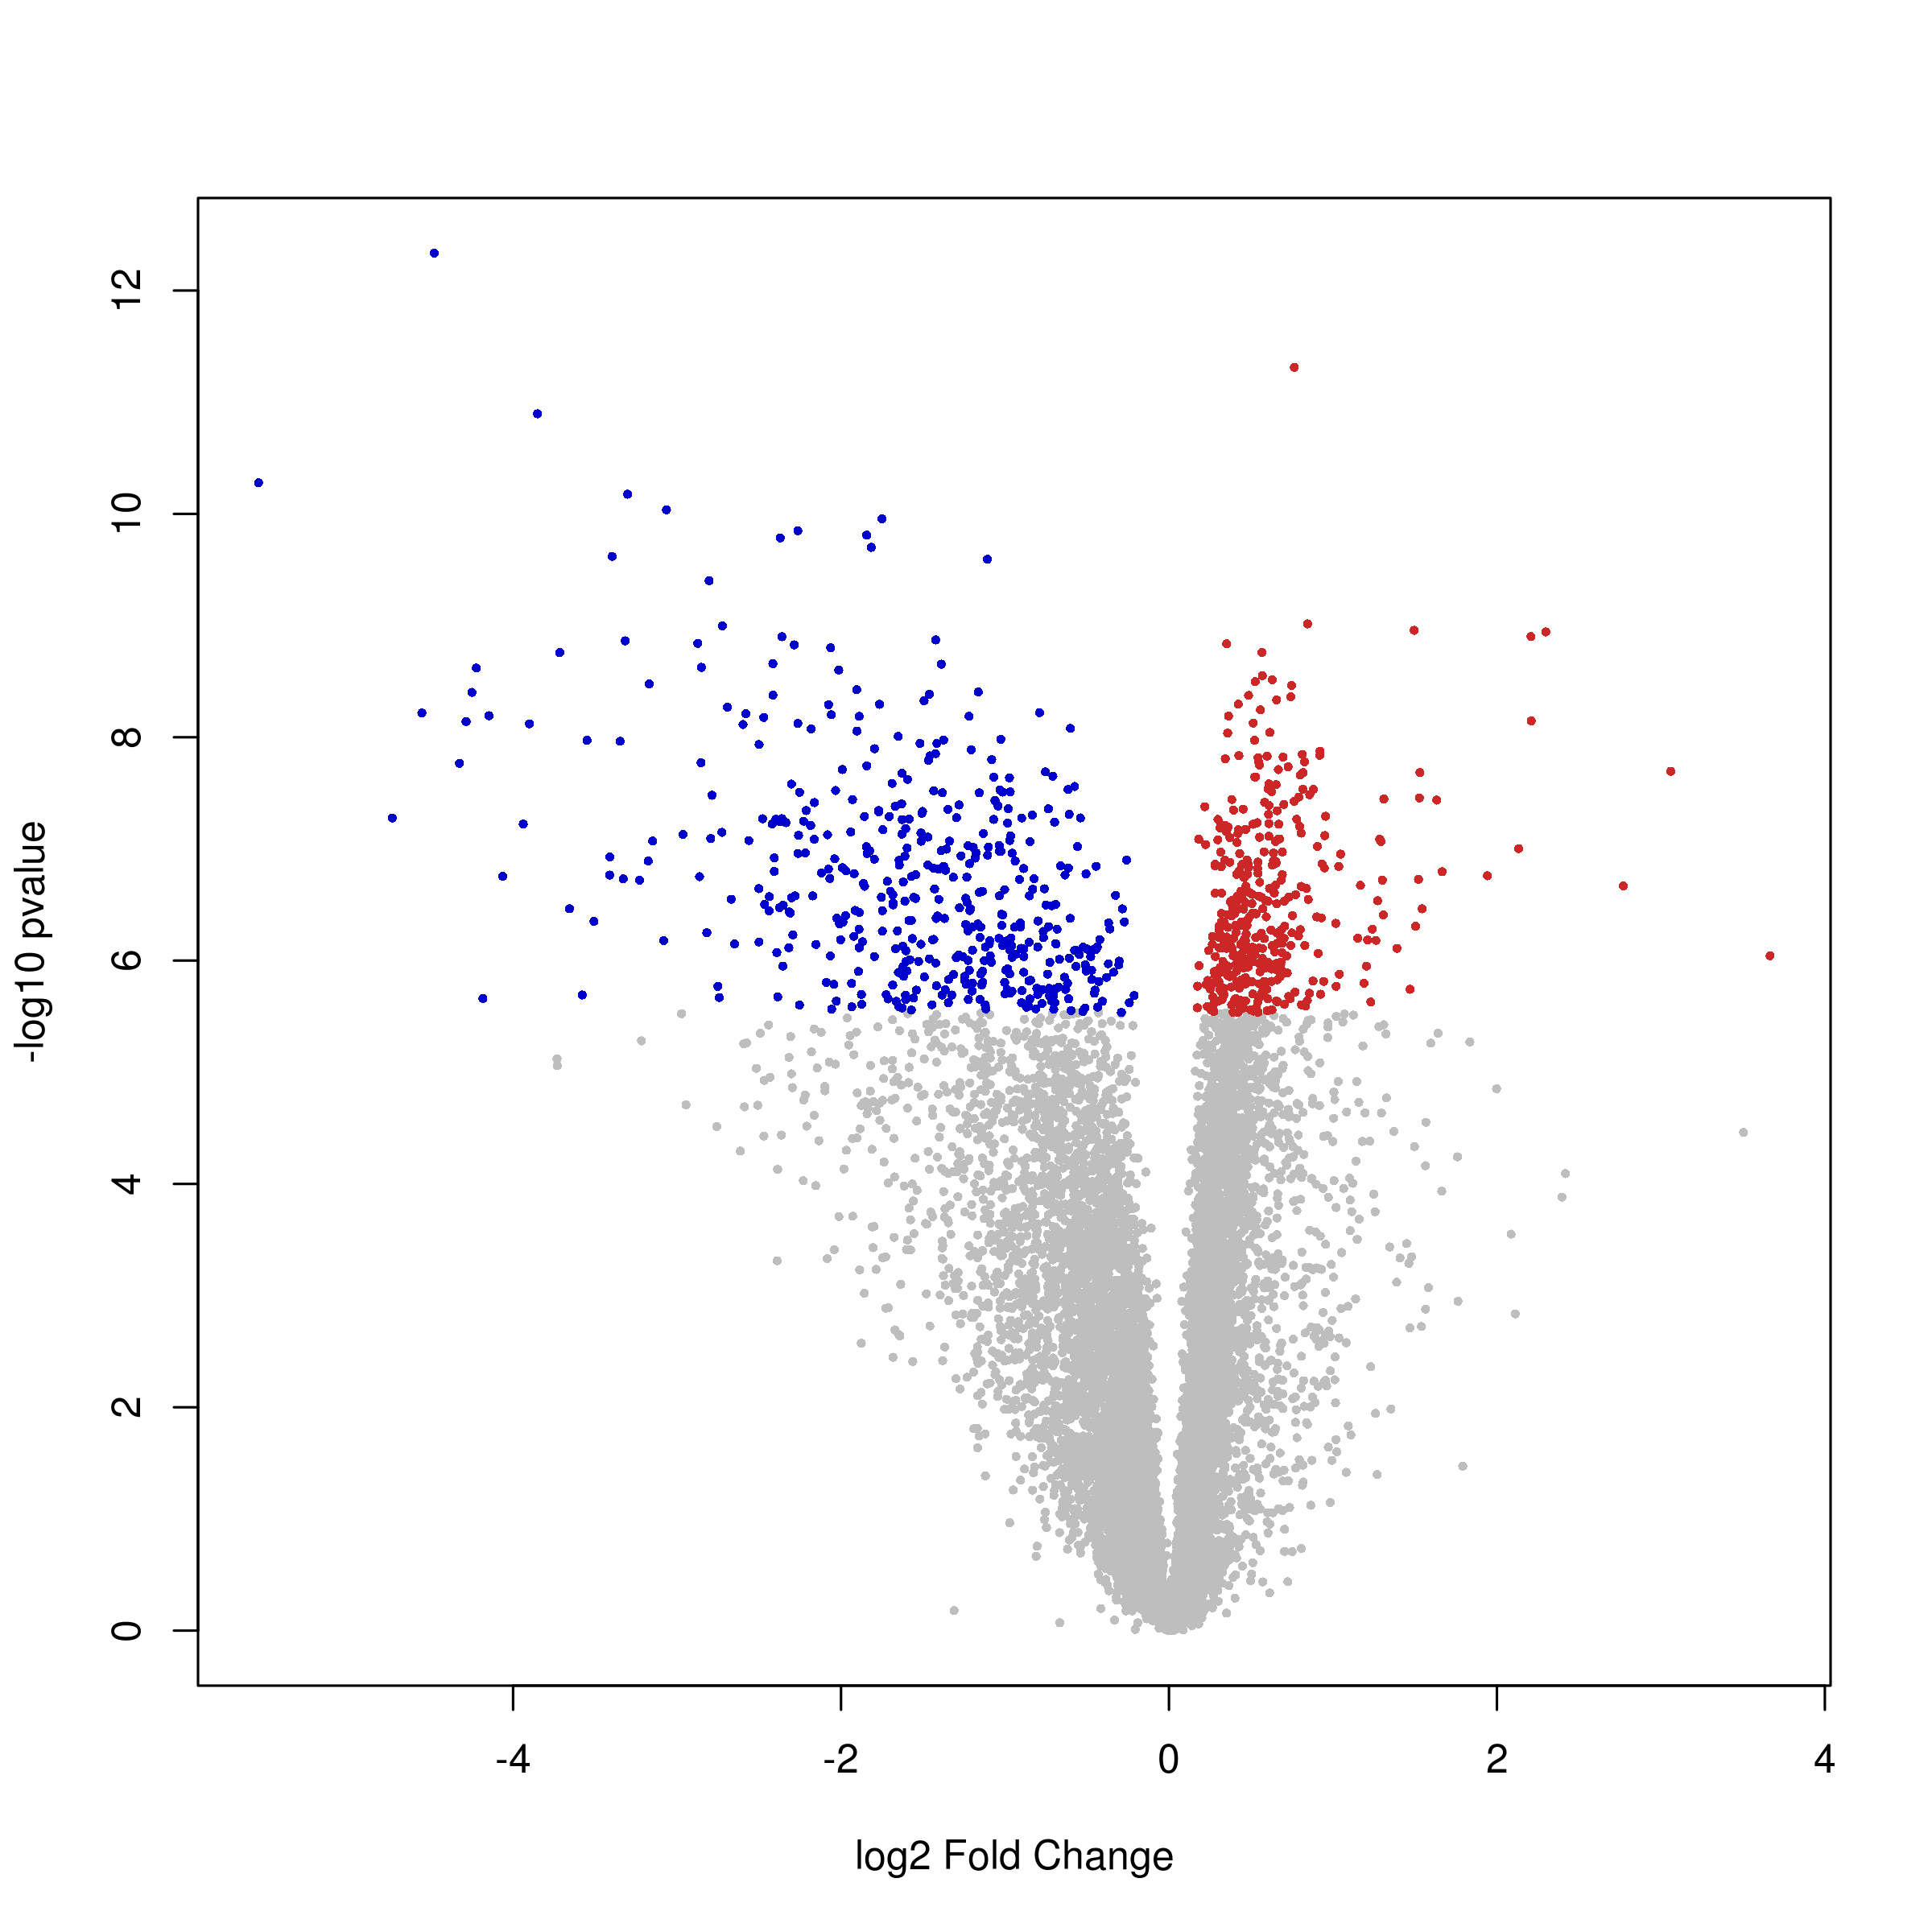
\includegraphics[width=0.45\textwidth]{environmental_risk/image/er_combat_volcano.png}
	}
	\caption[Volcano Plot]{Volcano plot of Case (PolyI:C) vs Control (Saline). 
		Genes that were significantly down-regulated are colored in blue whereas genes that were significantly up-regulated are colored in red. 
		a) Using only RNA-Seq data; 
		b) Using combination of RNA-Seq and microarray data.
	}
\end{figure}


\subsubsection{Gene Ontology(GO) enrichment}
A total of 28 GO terms were significantly overrepresented in the list of DEGs, with 10 and 18 GO terms represented by up- and down-regulated genes respectively, at a Bonferroni corrected p-value $<$ 0.05 (Table \ref{tab:geneOntologyFull}). 
Among the significant GO terms, a number of them, such as ``Developmental process'' (p-value $= 9.75\times 10^{-6}$), ``Regulation of neurogenesis'' (p-value $= 7.08\times 10^{-17}$) and ``Regulation of neurotransmitter levels'' (p-value $= 1.05\times 10^{-9}$) are related to brain function and development.

\subsubsection{Gene set enrichment}
Of the 149 gene sets tested, 27 were significantly enriched by the DEGs at a Bonferroni corrected p-value $<$ 0.05, including post-synaptic density protein and gene sets related to neurodevelopmental disorders, such as schizophrenia probable and autism associated modules (Table \ref{tab:fullGeneSetEnrichment}).

\subsection{Differential gene expression analysis with external controls}
We incorporated the external micro-array data as additional controls.
After quality control (QC), there are a total of 13,112 genes that can be found in both our RNA Seq data and the microarray chips.
Among the 13,112 genes, 868 were found to be differentially expressed (398 up-regulated and 470 down-regulated) with a Bonferroni-corrected p-value $<$ 0.05.
A volcano plot of PolyI:C versus Saline for all genes passing QC is presented in Figure \ref{subfig2:combatVoc}. 851 of the DEGs (98.0$\%$) overlapped with those discovered in our previous analysis without these external control data. 
Seven of the candidate schizophrenia genes previously identified by the PGC remained in our DEG list, including the GABA enzyme, \textit{Gad1} and \textit{Gad2}; \textit{Gabra3}, \textit{Ctnna2} and the dopamine-related gene, \textit{Th} (Table \ref{tab:candidateGeneTable}). 

\subsubsection{Gene Ontology enrichment}
The GO enrichment analysis found a total of 24 significantly enriched GO terms, of which 8 were enriched by the up-regulated genes and 16 were enriched by those down-regulated.
21 of them (87.5$\%$) overlapped with those found in the previous analysis without these external control data. ``Regulation of neurogenesis'' (enrichment p-value $= 4.94\times10^{-5}$) and ``Regulation of neurotransmitter levels'' (enrichment p-value $= 1.4\times10^{-7}$) were still among the enriched GO terms. 
\subsubsection{Gene set enrichment}
The gene-set enrichment analysis identified 5 enriched brain-related gene sets in the DEGs (Table \ref{tab:targetGeneSetEnrichment}), which were all identified in the previous analysis without these external control data. 
% Table generated by Excel2LaTeX from sheet 'Sheet1'
\afterpage{
\setlength\LTcapwidth{\textwidth}
\begin{longtable}{rrrrrr}
	\caption{Candidate genes for schizophrenia. We compared the candidate genes generated from the Psychiatric Genomic Consortium\cite{Greenwood2011} with the differentially expressed genes list from our study. It was found that majority (hyper geometric p-value $= 1.12\times 10^{-11}$) of the candidate genes were differentially expressed upon exposed to early maternal immune activation. Seven of the candidate genes remained in our differentially expressed gene list even after including the external control. Here only those that were significantly differentiated were shown}\label{tab:candidateGeneTable}\\
    \toprule
    \multicolumn{1}{c}{\multirow{2}[4]{*}{\textbf{Gene Name}}} & \multicolumn{3}{r}{Without external controls} &       & With external controls* \\
    \multicolumn{1}{c}{} & baseMean & Log2 Fold Change & Bonferroni Corrected P &       & Bonferroni Corrected P \\
    \midrule
    \textit{Adra2a} & 132.01 & -1.41 & $1.32\times 10^{-9}$ &       & 0.269 \\
    \textit{Adrbk2} & 400.52 & -0.343 & $1.77\times 10^{-3}$ &       & 1 \\
    \textit{Akt1} & 8537.11 & 0.0816 & 0.0364 &       & 1 \\
    \textit{Aspm} & 4875.21 & -0.179 & 0.017 &       & 1 \\
    \textit{Cacng2} & 30.78 & -1.53 & $1.21\times 10^{-8}$ &       & 0.233 \\
    \textit{Camk2a} & 357.99 & -0.583 & $6.25\times 10^{-8}$ &       & 1 \\
    \textit{Chrna4} & 844.89 & -0.278 & 0.0456 &       & 1 \\
    \textit{Chrnb2} & 336.29 & -1.1  & $7.66\times 10^{-11}$ &       & 0.0122 \\
    \textit{Crhr2} & 15.57 & 0.844 & 0.0146 &       & 1 \\
    \textit{Ctnna2} & 825.55 & -0.732 & $1.23\times 10^{-8}$ &       & 0.649 \\
    \textit{Dbh} & 31.55 & -2.49 & $5.15\times 10^{-15}$ &       & 0.0768 \\
    \textit{Dgcr2} & 3710.98 & 0.228 & $1.22\times 10^{-5}$ &       & 1 \\
    \textit{Disc1} & 54.78 & -0.58 & $1.05\times 10^{-3}$ &       & NA \\
    \textit{Dlg4} & 1626.55 & -0.353 & $2.45\times 10^{-11}$ &       & 0.0596 \\
    \textit{Drd2} & 12.38 & -0.974 & $7.79\times 10^{-3}$ &       & 1 \\
    \textit{Dtnbp1} & 1088.18 & 0.268 & $5.70\times 10^{-5}$ &       & 1 \\
    \textit{Ebf2} & 1003.45 & -0.451 & 0.025 &       & 1 \\
    \textit{Eea1} & 983.87 & -0.245 & $2.08\times 10^{-3}$ &       & 1 \\
    \textit{Erbb4} & 291.96 & -0.836 & $1.12\times 10^{-7}$ &       & 0.0912 \\
    \textit{Fez1} & 2783.05 & -0.581 & $4.68\times 10^{-11}$ &       & 1 \\
    \textit{Gabra3} & 204.37 & -0.634 & $1.67\times 10^{-8}$ &       & 0.00294 \\
    \textit{Gabrb2} & 150.74 & -1.137 & $4.73\times 10^{-17}$ &       & 0.0618 \\
    \textit{Gad1} & 80.15 & -2.96 & $2.79\times 10^{-19}$ &       & 0.00127 \\
    \textit{Gad2} & 183.28 & -1.66 & $1.25\times 10^{-13}$ &       & 0.0398 \\
    \textit{Grid2} & 15.99 & -0.933 & $2.76\times 10^{-3}$ &       & 1 \\
    \textit{Grik4} & 92.8  & -0.675 & $8.44\times 10^{-6}$ &       & 1 \\
    \textit{Grin3a} & 49.81 & -0.524 & $8.88\times 10^{-3}$ &       & 1 \\
    \textit{Grm2} & 250.43 & -0.673 & $3.66\times 10^{-4}$ &       & 1 \\
    \textit{Grm3} & 32.98 & -0.822 & $1.22\times 10^{-3}$ &       & 1 \\
    \textit{Grm4} & 164.28 & -0.659 & $7.32\times 10^{-5}$ &       & 1 \\
    \textit{Gsk3b} & 5068.93 & -0.197 & $6.37\times 10^{-4}$ &       & 1 \\
    \textit{Htr1b} & 121.93 & 0.448 & $9.74\times 10^{-4}$ &       & 1 \\
    \textit{Kcnh2} & 835.89 & -0.18 & 0.016 &       & 1 \\
    \textit{Ncam1} & 728.17 & -0.832 & $1.57\times 10^{-7}$ &       & 1 \\
    \textit{Nde1} & 6430.74 & 0.107 & $1.81\times 10^{-3}$ &       & 1 \\
    \textit{Ndel1} & 1195.39 & 0.114 & 0.0293 &       & 1 \\
    \textit{Nos1ap} & 109.8 & -0.579 & $3.86\times 10^{-5}$ &       & 1 \\
    \textit{Notch4} & 532.12 & -0.387 & $1.38\times 10^{-5}$ &       & 1 \\
    \textit{Ppp3cc} & 120.61 & -0.485 & $4.38\times 10^{-5}$ &       & 1 \\
    \textit{Prodh} & 550.47 & 0.699 & $7.59\times 10^{-13}$ &       & 0.807 \\
    \textit{Rgs4} & 164.1 & -0.958 & 0.0127 &       & 1 \\
    \textit{Slc1a2} & 777.36 & -1.28 & $4.82\times 10^{-21}$ &       & $6.92\times 10^{-3}$ \\
    \textit{Slc32a1} & 44.4  & -4.56 & $1.03\times 10^{-27}$ &       & $1.04\times 10^{-3}$ \\
    \textit{Slc6a1} & 126.37 & -1.88 & $3.32\times 10^{-18}$ &       & 0.341 \\
    \textit{Slc6a4} & 15.86 & -1.12 & $5.41\times 10^{-3}$ &       & 1 \\
    \textit{Sp4} & 910.49 & -0.407 & $4.15\times 10^{-11}$ &       & 0.063 \\
    \textit{Th} & 87.29 & -2.16 & $1.34\times 10^{-16}$ &       & $6.59\times 10^{-3}$ \\
    \textit{Ywhae} & 36516.86 & 0.258 & $1.32\times 10^{-6}$ &       & 1 \\
    \bottomrule
    \multicolumn{6}{l}{* Genes not found in the external control data were marked with NA} \\
    
\end{longtable}%
}

% Table generated by Excel2LaTeX from sheet 'Sheet2'
\afterpage{
\begin{landscape}
\setlength\LTcapwidth{\textwidth}
\begin{longtable}{cp{3cm}cccccp{5cm}}
  \caption{Gene Ontology(GO) enrichment Result. GOrilla and REViGO were used to perform GO enrichment analysis. Similar GO terms were clustered together and represented by a single representative GO terms. Here, only the representative GO terms were shown. }\label{tab:geneOntologyFull}\\
    \toprule
    \multicolumn{1}{c}{} & \multicolumn{3}{r}{\textit{\textbf{RNA-seq gene level}}} &  & \multicolumn{3}{r}{\textit{\textbf{Microarray and RNA-seq combined}}} \\
    \midrule
    \multicolumn{1}{c}{} & \multicolumn{3}{r}{\textit{\textbf{GO functional enrichment}}} & \textit{\textbf{}} & \multicolumn{3}{r}{\textit{\textbf{GO functional enrichment}}} \\
    \textit{\textbf{GO ID}} & \textit{\textbf{GO term}} & \textit{\textbf{P-value}} & \textit{\textbf{Direction}} & \textit{\textbf{}} & \textit{\textbf{Minimum P-value}} & \textit{\textbf{Direction}} & \textit{\textbf{Represented by}} \\
    GO:0007610 & behavior & $9.67\times 10^{-19}$ & Down  &       & $6.76\times 10^{-8}$ & Down & defense response \\
    GO:0022610 & biological adhesion & $4.65\times 10^{-10}$ & Down  &       & $8.66\times 10^{-5}$ & Down  &  \\
    GO:0065007 & biological regulation & $2.15\times 10^{-18}$ & Down  &       & $1.97\times 10^{-8}$ & Down  &  \\
    GO:0001775 & cell activation & $5.56\times 10^{-7}$ & Down  &       & $4.96\times 10^{-10}$ & Down  &  \\
    GO:0007155 & cell adhesion & $6.12\times 10^{-10}$ & Down  &       & $7.97\times 10^{-5}$ & Down  &  \\
    GO:0007049 & cell cycle & $9.99\times 10^{-3}$ & Up    &       & -     & -     &  \\
    GO:0008283 & cell proliferation & $5.53\times 10^{-3}$ & Up    &       & $1.83\times 10^{-3}$ & Up    &  \\
    GO:0008037 & cell recognition & $6.05\times 10^{-3}$ & Down  &       & $5.28\times 10^{-3}$ & Down  &  \\
    GO:0007267 & cell-cell signaling & $5.9\times 10^{-6}$ & Down  &       & -     & -     &  \\
    GO:0006928 & cellular component movement & $1.40\times 10^{-7}$ & Down  &       & $1.74\times 10^{-5}$ & Down  &  \\
    GO:0071840 & cellular component organization or biogenesis & $4.01\times 10^{-6}$ & Up    &       & -     & -     &  \\
    GO:0009987 & cellular process & $9.23\times 10^{-13}$ & Up    &       & $1.57\times 10^{-3}$ & Up    &  \\
    GO:0006974 & cellular response to DNA damage stimulus & $4.76\times 10^{-3}$ & Up    &       & -     & -     &  \\
    GO:0032502 & developmental process & $1.23\times 10^{-5}$ & Down  &       & -     & -     &  \\
    GO:0002376 & immune system process & $1.16\times 10^{-8}$ & Down  &       & $4.39\times 10^{-11}$ & Down  &  \\
    GO:0051703 & intraspecies interaction between organisms & $1.48\times 10^{-3}$ & Down  &       & -     & -     &  \\
    GO:0040011 & locomotion & $2.10\times 10^{-9}$ & Down  &       & $7.23\times 10^{-6}$ & Down  &  \\
    GO:1903047 & mitotic cell cycle process & $1.94\times 10^{-3}$ & Up    &       & -     & -     &  \\
    GO:0032501 & multicellular organismal process & $1.61\times 10^{-11}$ & Down  &       & -     & -     &  \\
    GO:0051704 & multi-organism process & $6.29\times 10^{-3}$ & Down  &       & -     & -     &  \\
    GO:0001890 & placenta development & $9.63\times 10^{-5}$ & Up    &       & $4.01\times 10^{-5}$ & Up    & osteoblast differentiation \\
    GO:0042391 & regulation of membrane potential & $1.79\times 10^{-9}$ & Down  &       & $1.40\times 10^{-7}$ & Down  & regulation of neurotransmitter levels \\
    GO:0050767 & regulation of neurogenesis & $3.54\times 10^{-17}$ & Down  &       & $6.82\times 10^{-11}$ & Down  & cell projection organization, cognition, immune effector process, regulation of multicellular organismal process \\
    \multicolumn{1}{c}{GO:0022613} & ribonucleoprotein complex biogenesis & \multicolumn{1}{c}{$1.02\times 10^{-27}$} & \multicolumn{1}{c}{Up} & \multicolumn{1}{c}{} & \multicolumn{1}{c}{$6.37\times 10^{-13}$} & \multicolumn{1}{c}{Up} &  \\
    \multicolumn{1}{c}{GO:0006396} & RNA processing & \multicolumn{1}{c}{$2.25\times 10^{-50}$} & \multicolumn{1}{c}{Up} & \multicolumn{1}{c}{} & \multicolumn{1}{c}{$5.18\times 10^{-15}$} & \multicolumn{1}{c}{Up} & translation \\
    \multicolumn{1}{c}{GO:0050658} & RNA transport & \multicolumn{1}{c}{$3.21\times 10^{-10}$} & \multicolumn{1}{c}{Up} & \multicolumn{1}{c}{} & \multicolumn{1}{c}{$1.17\times 10^{-3}$} & \multicolumn{1}{c}{Up} &  \\
    \multicolumn{1}{c}{GO:0023052} & signaling & \multicolumn{1}{c}{$4.36\times 10^{-9}$} & \multicolumn{1}{c}{Down} & \multicolumn{1}{c}{} & \multicolumn{1}{c}{-} & \multicolumn{1}{c}{-} &  \\
    \multicolumn{1}{c}{GO:0071353} & cellular response to interleukin-4 & \multicolumn{1}{c}{-} & \multicolumn{1}{c}{-} & \multicolumn{1}{c}{} & \multicolumn{1}{c}{$2.20\times 10^{-5}$} & \multicolumn{1}{c}{Up} &  \\
    \multicolumn{1}{c}{GO:0000082} & G1/S transition of mitotic cell cycle & \multicolumn{1}{c}{-} & \multicolumn{1}{c}{-} & \multicolumn{1}{c}{} & \multicolumn{1}{c}{$6.14\times 10^{-3}$} & \multicolumn{1}{c}{Up} &  \\
    \multicolumn{1}{c}{GO:0030001} & metal ion transport & \multicolumn{1}{c}{-} & \multicolumn{1}{c}{-} & \multicolumn{1}{c}{} & \multicolumn{1}{c}{$1.25\times 10^{-7}$} & \multicolumn{1}{c}{Down} &  \\
    \multicolumn{1}{c}{GO:0050896} & response to stimulus & \multicolumn{1}{c}{-} & \multicolumn{1}{c}{-} & \multicolumn{1}{c}{} & \multicolumn{1}{c}{$9.89\times 10^{-7}$} & \multicolumn{1}{c}{Down} &  \\
    \bottomrule
    \end{longtable}%
    
\end{landscape}
}
% Table generated by Excel2LaTeX from sheet 'Sheet3'
\begin{landscape}
\begin{table}[htbp]
  \centering
  \caption{Gene set enrichment results of differential expressed genes combining microarray and RNA Seq data.
  Enrichment results mapping to \textit{de-novo} mutations and common variants are also shown.
  It was noted that the Post-synaptic density protein (PSD) gene sets were enriched with \textit{de-novo} mutations from 3 out of 4 studies and only the microglia gene set was enriched by the common variants observed in the schizophrenia Genome-wide association study (GWAS) conducted by the Psychiatric Genomic Consortium\cite{Ripke2013}.}
    \begin{tabular}{cccccccc}
    \multicolumn{1}{c}{\multirow{3}[3]{*}{\textbf{Gene Set}}} & \multicolumn{1}{c}{\multirow{3}[3]{*}{\textbf{RNA Seq}}} & \textbf{Denovo } & \textbf{} & \textbf{} & \textbf{} & \textbf{GWAS} & \textbf{} \\
    \cline{3-8}
    
    \multicolumn{1}{c}{} & \multicolumn{1}{c}{} & 
    \multicolumn{1}{p{2.3cm}}{\multirow{2}[2]{*}{\textbf{Fromer et al.}}} & \multicolumn{1}{p{2cm}}{\multirow{2}[2]{*}{\textbf{Neale et al.}}} & \multicolumn{1}{p{2.4cm}}{\multirow{2}[2]{*}{\textbf{Sanders et al.}}} & \multicolumn{1}{p{2.3cm}}{\multirow{2}[2]{*}{\textbf{O'Roak et al.}}} & \multicolumn{1}{p{2.3cm}}{\multirow{2}[2]{*}{\textbf{Anney et al.}}} & \multicolumn{1}{p{2.3cm}}{\multirow{2}[2]{*}{\textbf{Ripke et al.}}} \\[0.25cm]
    \multicolumn{1}{c}{} & \multicolumn{1}{c}{} & \multicolumn{1}{c}{\textbf{Scz\cite{Fromer2014}}} & \multicolumn{1}{c}{\textbf{ASD\cite{Neale2012}}} & \multicolumn{1}{c}{\textbf{ASD\cite{Sanders2012}}} & \multicolumn{1}{c}{\textbf{ASD\cite{ORoak2012}}} & \multicolumn{1}{c}{\textbf{ASD\cite{Anney2010a}}} & \multicolumn{1}{c}{\textbf{Scz\cite{Ripke2013}}} \\
    \midrule
    Neuron definite\cite{Cahoy2008} & $2.66\times 10^{-4}$ & 0.358 & 0.381 & 1     & $3.83\times10^{-3}$ & 0.614 & 0.188 \\
    Neuron probable\cite{Cahoy2008} & $5.77\times10^{-3}$ & $7.14\times10^{-9}$ & 0.373 & 1     & $2.51\times10^{-7}$ & 0.763 & 0.323 \\
    Microglia (Type1)\cite{Miller2010} & $3.17\times10^{-8}$ & 1     & 1     & 1     & 1     & 0.938 & $9.64\times10^{-3}$ \\
    PSD proteins\cite{Bayes2011} & $3.54\times10^{-5}$ & $3.07\times10^{-10}$ & 0.0732 & $2.63\times10^{-3}$ & $3.35\times10^{-4}$ & 0.461 & 0.548 \\
    Ribosome\cite{Miller2010} & $9.41\times10^{-4}$ & 1     & 1     & 1     & 1     & 0.489 & 0.317 \\
    \bottomrule
    \end{tabular}%
  \label{tab:targetGeneSetEnrichment}%
\end{table}%
\end{landscape}


\begin{figure}
	\caption[rtPCR Results]{real time PCR validation of RNA Seq results.
		The delta CT values are highly correlated with the RNA-Seq counts (case: pearson correlation = -0.968, control: pearson correlation = 0.952), suggesting that the RNA-Seq count is a true representation of the RNA concentration.
		The difference in detla CT between the cases and controls also support the differential gene expression results of the RNA Sequencing analysis.}\label{fig:rtResult}
		\vspace{-20pt}
	\begin{center}
		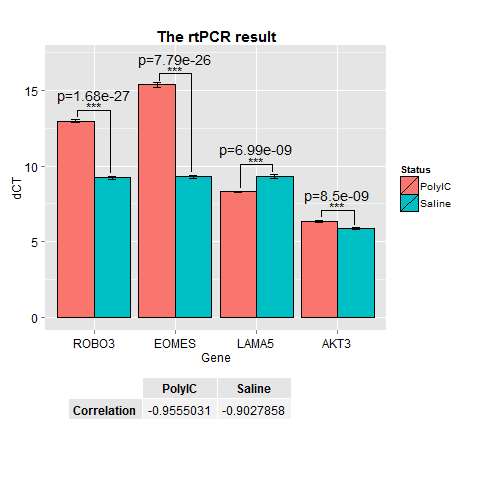
\includegraphics[trim=0cm 2cm 0cm 1cm, clip=true, width=0.7\textwidth]{environmental_risk/image/er_rtPCR.png}
	\end{center}
\end{figure}

\subsection{Test for burden of genetic risk variants in enriched brain-related gene sets in schizophrenia and autism cohorts }
Among the 27 enriched brain-related gene sets identified in the analysis without external control (Table \ref{tab:fullGeneSetEnrichment}), three (``Post-synaptic Density Proteins'', ``Neuron Probable'' and ``Down with Alzheimer's'') were enriched with rare \textit{de-novo} mutations in more than one study. 
In addition, the ``Oligodendrocyte Marker'' gene set was enriched with both rare \textit{de-novo} mutations and common genetic variants in schizophrenia studies. 

When combined with external control, only 5 gene sets remained \ref{tab:targetGeneSetEnrichment}. 
Of the 5 remaining gene sets, only the microglia gene set from \citet{Miller2010} was found to contain significantly more common genetic variations associated with schizophrenia in the PGC genome wide association study (GWAS).
Whereas the significant ``Neuron Probable'' and ``Post-synaptic Density Proteins'' were among the 5 remaining gene sets.

\subsection{RT-PCR validation of RNA-Seq data}
The CT value is the unit used during rtPCR to indicates the mRNA concentration.
A high CT value means more PCR cycle is required to detect the mRNA, therefore indicating a low mRNA concentration.
Thus, a high CT value represent a low mRNA concentration and a low CT value represent a high mRNA concentration, as oppose to the RNA Seq count value.

In the rtPCR, the CT values were highly negatively correlated with the RNA-Seq (Case: r  = -0.968, p = $2.98\times10^{-15}$; Control: r  = -0.952, p= $2.834\times10^{-13}$), suggesting that the RNA-Seq counts truly reflected the true mRNA concentration (Figure \ref{fig:rtResult}). 
Simple T-test performed on the relative CT values confirmed that all genes tested were significantly differentially expressed (Figure \ref{fig:rtResult}).


	
\subsection{Alternative splicing}
\subsection{De-novo Assembly}

\section{Discussion}
\section{Conclusion}
\section{Supplementary Materials}
% Table generated by Excel2LaTeX from sheet 'Sheet1'
\begin{table}[htbp]
  \centering
  \caption{Primer Sequences used in real time PCR}
    \begin{tabular}{rr}
    \toprule
    Gene Name & Primer Sequence \\
    \midrule
    \gene{Actb}  & ACTGAGCTGCGTTTTACACCCTTTC \\
    \gene{Akt3}  & CTTCTCAGTGGCAAAATGTCAGTTA \\
    \gene{Eomes} & AATAACATGCAGGGCAATAAGATGT \\
    \gene{Lama5} & ACACGAGCGAGACCAGTGAGAAGAT \\
    \gene{Robo3} & AAGGGAGTCAAGTCCTGCTTTTCCC \\
    \bottomrule
    \end{tabular}%
  \label{suppleTab:rtPCR}%
\end{table}%


\chapter{Genetic risk factors of Neurodevelopmental disorders}
\section{Introduction}
\subsection{Heritability estimate}
\subsubsection{Heritability explained by Common SNPs}
\subsubsection{Missing Heritability}
\subsubsection{Risk Prediction}
\subsection{Challenge of heritability estimation}
\section{Methodology}
\subsection{Estimation of heritability using test-statistic}
\subsection{Simulation}
\subsubsection{Quantitative Traits}
\paragraph{Genome Wide Association Studies}
\paragraph{Exome Sequencing / Targeted Sequencing}
\subsubsection{Case Control Studies}
\subsection{Comparing with existing software}
\subsubsection{Quantitative Traits}
\paragraph{Genome Wide Association Studies}
\paragraph{Exome Sequencing / Targeted Sequencing}
\subsubsection{Case Control Studies}

\subsection{Estimate the heritability of neurodevelopmental disorders}
\section{Result}
\section{Discussion}



\section{Conclusion}


\chapter{Summary and Conclusion}


\printbibliography

\chapter*{Appendix}
\end{document}